\documentclass[11pt]{article}
\usepackage{amssymb}
\usepackage{amsmath}
\usepackage{amssymb}
\usepackage{amsmath}
\usepackage{tikz}
\usetikzlibrary{arrows,shapes.geometric,positioning}

\begin{document}

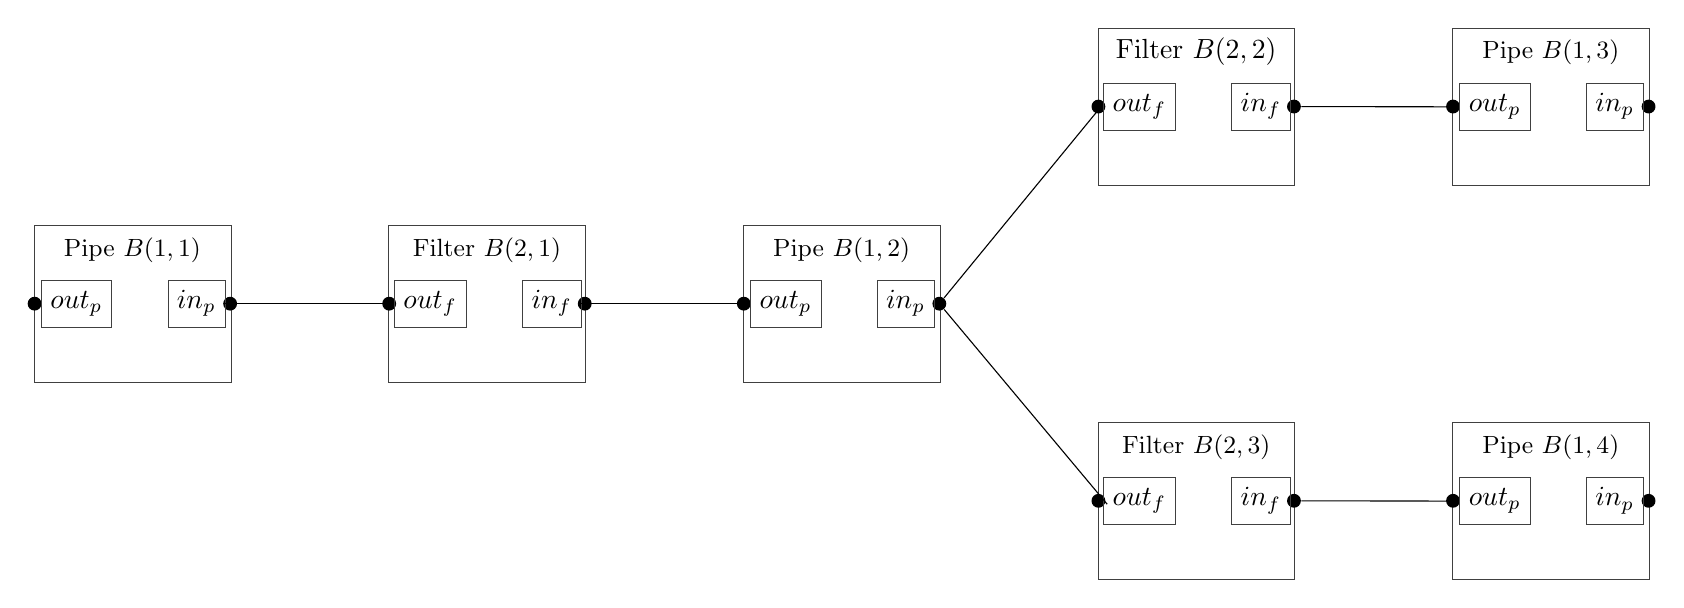
\begin{tikzpicture}[>=stealth',shorten >=1pt,auto,node distance=1cm,baseline=(current bounding box.north)]
					\tikzstyle{component}=[rectangle,ultra thin,draw=black!75,align=center,inner sep=9pt,minimum size=1.5cm,minimum width=2.5cm,minimum height=2cm]
					\tikzstyle{port}=[rectangle,ultra thin,draw=black!75,minimum size=6mm]
					\tikzstyle{bubble} = [fill,shape=circle,minimum size=5pt,inner sep=0pt]
					\tikzstyle{type} = [draw=none,fill=none] 
					
					
					\node [component] (a1) {};
					
					\node[bubble] (a2) [right=-0.105cm of a1]   {};   
					\node [port] (a3) [right=-0.805cm of a1]  {$in_p$};  
					
					
					
					\node[bubble] (a4) [left=-0.105cm of a1]   {};   
					\node [port] (a5) [left=-0.99cm of a1]  {$out_p$};  
					
					\node[type]  [above=-0.6cm of a1]{{\small Pipe $B(1,1)$}};
					
					
					
					\node [component] (b2) [right=2cm of a1]  {};
					\node[bubble] (b3) [right=-0.105cm of b2]   {};   
					\node [port] (b4) [right=-0.805cm  of b2]  {$in_f$};  
					
					
					
					\node[bubble] (b5) [left=-0.105cm of b2]   {};   
					\node [port] (b6) [left=-0.99cm of b2]  {$out_f$};  
					
					\node[type]  [above=-0.6cm of b2]{{\small Filter $B(2,1)$}};
					\path[-]          (a3)  edge                  node {} (b6);
					
					
					\node [component] (c2) [right=2cm of b2]{};
					
					\node[bubble] (c3) [right=-0.105cm of c2]   {};   
					\node [port] (c4) [right=-0.805cm  of c2]  {$in_p$};  
					
					
					
					\node[bubble] (c5) [left=-0.105cm of c2]   {};   
					\node [port] (c6) [left=-0.99cm of c2]  {$out_p$};  
					
					\node[type]  [above=-0.6cm of c2]{{\small Pipe $B(1,2)$}};
					
					\path[-]          (b4)  edge                  node {} (c6);
					
					
					\node [component] (d2) [above right= 0.5cm and 2cm of c2]  {};
					\node[bubble] (d3) [right=-0.105cm of d2]   {};  
					\node [port] (d4) [right=-0.805cm  of d2]  {$in_f$};  
					
					
					
					\node[bubble] (d5) [left=-0.105cm of d2]   {};   
					\node [port] (d6) [left=-0.99cm of d2]  {$out_f$};  
					\node[] (i1) [above left=-0.3 cm and -0.20cm of d6]   {};
					
					\node[type]  [above=-0.6cm of d2]{Filter $B(2,2)$};
					\path[-]          (c3)  edge                  node {} (i1);
					
					
					\node [component] (e2) [below right= 0.5cm and 2cm of c2]  {};
					\node[bubble] (e3) [right=-0.105cm of e2]   {};   
					\node [port] (e4) [right=-0.805cm  of e2]  {$in_f$};  
					
					
					
					\node[bubble] (e5) [left=-0.105cm of e2]   {};   
					\node [port] (e6) [left=-0.99cm  of e2]  {$out_f$}; 
					\node[] (i2) [above left=-0.62 cm and -0.30cm of e6]   {};
					
					
					
					\node[type]  [above=-0.6cm of e2]{{\small Filter $B(2,3)$}};
					\path[-]          (c3)  edge                  node {} (i2);
					
					
					\node [component] (f2) [right=2cm of d2]{};
					
					\node[bubble] (f3) [right=-0.105cm of f2]   {};   
					\node [port] (f4) [right=-0.805cm  of f2]  {$in_p$}; 
					
					
					
					\node[bubble] (f5) [left=-0.105cm of f2]   {};   
					\node [port] (f6) [left=-0.99cm  of f2]  {$out_p$};  
					\node[] (i3) [above left=-0.43 cm and -0.25cm of f6]   {};
					
					
					
					\node[type]  [above=-0.6cm of f2]{{\small Pipe $B(1,3)$}};
					
					\path[-]          (d3)  edge                  node {} (i3);
					
					\node [component] (g2) [right=2cm of e2]{};
					
					\node[bubble] (g3) [right=-0.105cm of g2]   {};   
					\node [port] (g4) [right=-0.805cm  of g2]  {$in_p$};  
					
					
					\node[bubble] (g5) [left=-0.105cm of g2]   {};   
					\node [port] (g6) [left=-0.99cm  of g2]  {$out_p$};  
					\node[] (i4) [above left=-0.43 cm and -0.25cm of g6]   {};
					
					
					\node[type]  [above=-0.6cm of g2]{{\small Pipe $B(1,4)$}};
					
					\path[-]          (e3)  edge                  node {} (i4);
					
			\end{tikzpicture}

\end{document}